\documentclass[border=3pt]{standalone}
% Preâmbulo compartilhado pelos diagramas TikZ da aula 5 de IHC (Processos de Design)
\usepackage[T1]{fontenc}
\usepackage[utf8]{inputenc}
\usepackage{lmodern}
\usepackage{amsmath}
\usepackage{xcolor}
\usepackage{tikz}
\usetikzlibrary{arrows.meta,angles,quotes,decorations.pathmorphing,calc,
                positioning,shapes.geometric,shapes.misc,backgrounds,fit,
                math}

% Paleta (mesma dos SVGs originais)
% Paleta da disciplina de IHC: acento roxo (#755099), da capa do livro.
% (o nome "dblue" é mantido para não alterar todos os diagramas)
\definecolor{dblue}{HTML}{755099}
\definecolor{dorange}{HTML}{B3541E}
\definecolor{dgreen}{HTML}{4A7C59}
\definecolor{dred}{HTML}{9C4B4B}
\definecolor{dcream}{HTML}{F4F1EA}
\definecolor{dshade}{HTML}{DDD7C9}

% Função gaussiana (não normalizada por padrão de escala visual)
\pgfmathdeclarefunction{gauss}{3}{%
  \pgfmathparse{1/(#3*sqrt(2*pi))*exp(-((#1-#2)^2)/(2*#3^2))}%
}

% Estilos comuns (prefixo d... para não colidir com chaves internas do pgf)
\tikzset{
  >={Stealth[length=2mm]},
  dguide/.style={gray!55, dashed, line width=0.4pt},
  daxis/.style={gray!60, line width=0.7pt, ->},
  dbody/.style={fill=black!3, draw=black!80, line width=1pt},
  dacc/.style={draw=dblue, line width=1pt},
  dlbl/.style={black!55, font=\small},
  dsub/.style={black!45, font=\footnotesize},
  dstate/.style={circle, draw=black!80, fill=dcream, line width=1pt,
                 minimum size=17mm, font=\large, inner sep=1pt},
  dobs/.style={circle, draw=black!80, fill=dshade, line width=1pt,
               minimum size=14mm, font=\large, inner sep=1pt},
  dbox/.style={rounded corners=2pt, draw=black!80, fill=dcream, line width=1pt,
               align=center, inner sep=6pt},
  dop/.style={circle, draw=black!80, fill=white, line width=1pt,
              minimum size=6mm, inner sep=0pt, font=\small},
  dtrans/.style={->, dblue, line width=1pt},
  dmeas/.style={->, dorange, line width=1pt},
  dcurve/.style={line width=1pt, dblue},
  dcurveb/.style={line width=1.4pt, dorange},
}

\begin{document}
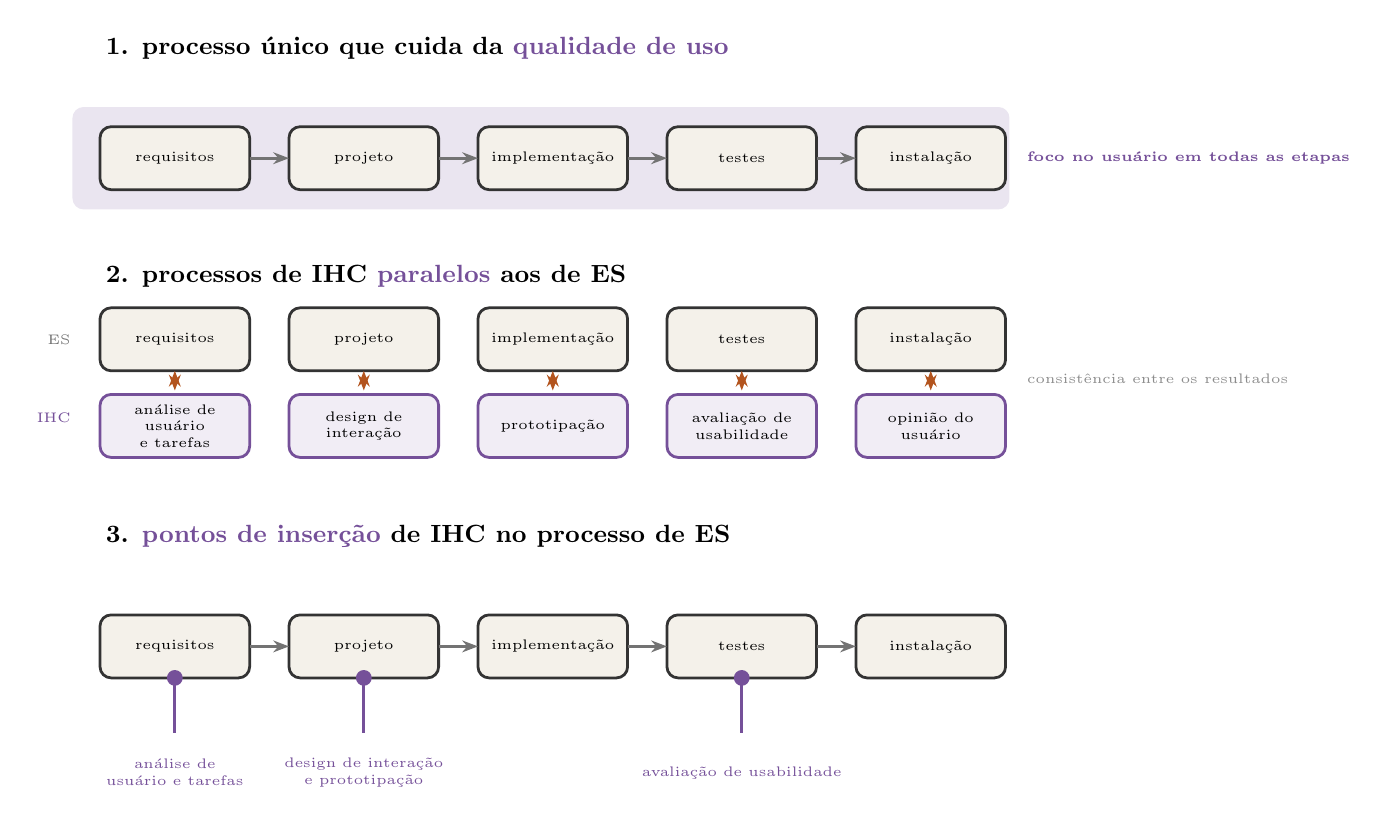
\begin{tikzpicture}[x=1cm,y=1cm,
   st/.style={dbox, rounded corners=4pt, minimum width=1.9cm, minimum height=0.8cm, font=\tiny, inner sep=2pt}]

  \fill[dblue!15, rounded corners=4pt] (-0.3,3.55) rectangle (11.6,4.85);
  % abordagem 1
  \node[font=\small\bfseries, anchor=west] at (0,5.6) {1. processo único que cuida da \textcolor{dblue}{qualidade de uso}};
  \foreach \i/\t in {0/requisitos,2.4/projeto,4.8/implementação,7.2/testes,9.6/instalação} { \node[st] at (\i+1.0,4.2) {\t}; }
  \draw[->, black!55, line width=1pt] (1.95,4.2) -- (2.45,4.2); \draw[->, black!55, line width=1pt] (4.35,4.2) -- (4.85,4.2); \draw[->, black!55, line width=1pt] (6.75,4.2) -- (7.25,4.2); \draw[->, black!55, line width=1pt] (9.15,4.2) -- (9.65,4.2);
  \node[dblue, font=\tiny\bfseries, anchor=west] at (11.7,4.2) {foco no usuário em todas as etapas};

  % abordagem 2
  \node[font=\small\bfseries, anchor=west] at (0,2.7) {2. processos de IHC \textcolor{dblue}{paralelos} aos de ES};
  \node[dlbl, font=\tiny, anchor=east] at (-0.2,1.9) {ES};
  \node[dlbl, font=\tiny, anchor=east, dblue] at (-0.2,0.9) {IHC};
  \foreach \i/\t/\u in {0/requisitos/{análise de usuário e tarefas},2.4/projeto/{design de interação},4.8/implementação/prototipação,7.2/testes/{avaliação de usabilidade},9.6/instalação/{opinião do usuário}} { \node[st] at (\i+1.0,1.9) {\t}; \node[st, draw=dblue, fill=dblue!10, text width=1.7cm, align=center] at (\i+1.0,0.8) {\u}; \draw[<->, dorange, line width=0.9pt] (\i+1.0,1.5) -- (\i+1.0,1.25); }
  \node[dsub, font=\tiny, anchor=west] at (11.7,1.4) {consistência entre os resultados};

  % abordagem 3
  \node[font=\small\bfseries, anchor=west] at (0,-0.6) {3. \textcolor{dblue}{pontos de inserção} de IHC no processo de ES};
  \foreach \i/\t in {0/requisitos,2.4/projeto,4.8/implementação,7.2/testes,9.6/instalação} { \node[st] at (\i+1.0,-2.0) {\t}; }
  \draw[->, black!55, line width=1pt] (1.95,-2.0) -- (2.45,-2.0); \draw[->, black!55, line width=1pt] (4.35,-2.0) -- (4.85,-2.0); \draw[->, black!55, line width=1pt] (6.75,-2.0) -- (7.25,-2.0); \draw[->, black!55, line width=1pt] (9.15,-2.0) -- (9.65,-2.0);
  \foreach \x/\t in {1.0/{análise de usuário e tarefas},3.4/{design de interação e prototipação},8.2/{avaliação de usabilidade}} {
    \draw[dblue, line width=1pt] (\x,-2.4) -- (\x,-3.1); \fill[dblue] (\x,-2.4) circle (0.1);
    \node[dblue, font=\tiny, align=center, text width=2.6cm] at (\x,-3.6) {\t};
  }

\end{tikzpicture}
\end{document}
